\question Os dados abaixo referem-se a dureza de 30 peças de alumínio
\begin{parts}
    \part Represente os dados por meio de uma gráfico de ramos-e-folhas.
    \begin{solution}
        Gráfico de Ramo-e-Folhas construido para valores inteiros(truncados) dos dados:
        \begin{table}[H]
            \centering
            \begin{tabular}{r|l@{\hspace{4 pt}}l@{\hspace{4 pt}}l@{\hspace{4 pt}}l@{\hspace{4 pt}}l@{\hspace{4 pt}}l@{\hspace{4 pt}}l@{\hspace{4 pt}}}
                5 & 1 & 1 & 2 & 3 & 3 & 4 & 4 \\
                5 & 5 & 6 & 6                 \\
                6 & 0 & 4 & 4                 \\
                6 & 7 & 9                     \\
                7 & 0 & 0 & 1 & 1 & 2 & 3 & 4 \\
                7 & 8 & 9                     \\
                8 & 3 & 3 & 4                 \\
                8 & 6 & 8                     \\
                9                             \\
                9 & 5                         \\
            \end{tabular}
        \end{table}
    \end{solution}
    \part Represente os dados por meio de uma distribuição de frequências.
    \begin{solution}
        Usando uma distribuição de frequências simples temos, temos:
        % latex table generated in R 4.3.3 by xtable 1.8-4 package
        % Thu Mar 21 20:32:51 2024
        \begin{table}[H]
            \centering
            \begin{tabular}{rlr}
                \hline
                   & Dureza & Freq \\
                \hline
                1  & 50.7   & 1    \\
                2  & 51.1   & 1    \\
                3  & 52.4   & 1    \\
                4  & 53     & 1    \\
                5  & 53.4   & 1    \\
                6  & 53.5   & 1    \\
                7  & 54.1   & 1    \\
                8  & 55.3   & 1    \\
                9  & 55.7   & 2    \\
                10 & 59.5   & 1    \\
                11 & 63.5   & 1    \\
                12 & 64.3   & 1    \\
                13 & 67.3   & 1    \\
                14 & 69.1   & 1    \\
                15 & 69.5   & 1    \\
                16 & 70.2   & 1    \\
                17 & 70.5   & 1    \\
                18 & 71.4   & 1    \\
                19 & 72.3   & 1    \\
                20 & 73     & 1    \\
                21 & 74.4   & 1    \\
                22 & 77.8   & 1    \\
                23 & 78.5   & 1    \\
                24 & 82.5   & 1    \\
                25 & 82.7   & 1    \\
                26 & 84.3   & 1    \\
                27 & 85.8   & 1    \\
                28 & 87.5   & 1    \\
                29 & 95.4   & 1    \\
                \hline
            \end{tabular}
        \end{table}

        Perceba que temos uma grande quantidade de elementos com frequência 1, o que indica que a \textbf{distribuição é bem dispersa}, assim seria mais adequado usar uma distribuição de frequência por intervalos.

        \begin{equation*}
            \begin{split}
                A_{total} & = x_n - x_1 = 95.4 - 50.7 = 44.7 \\
            \end{split}
        \end{equation*}

        Usando a regra da raiz quadrada para \textbf{calcular a quantidade de classes} $k$ temos:

        \begin{equation*}
            \begin{split}
                k & = \sqrt{29} = 5.385 \approx 5
            \end{split}
        \end{equation*}

        Usando a regra de Sturges temos:

        \begin{equation*}
            \begin{split}
                k & = 1 + 3.3 \log_{10}(29) = 1 + 3.3 \times 1.462 = 1 + 4.824 = 5.824 \approx 6 \\
            \end{split}
        \end{equation*}

        \pagebreak

        Usemos $k = 6$ \footnote{Motivo?}, assim temos o \textbf{cálculo da amplitude do intervalo} $h$ dado por:

        \begin{equation*}
            \begin{split}
                h = \frac{A_{total}}{k} = \frac{44.7}{6} = 7.45 \approx 7.4
            \end{split}
        \end{equation*}

        Dessa forma teremos a seguinte distribuição de frequências em intervalos:

        % latex table generated in R 4.3.3 by xtable 1.8-4 package
        % Thu Mar 21 21:20:14 2024
        \begin{table}[H]
            \centering
            \begin{tabular}{rlr}
                \hline
                  & intervals   & Freq \\
                \hline
                1 & [49.7,57.1) & 10   \\
                2 & [57.1,64.5) & 3    \\
                3 & [64.5,71.9) & 6    \\
                4 & [71.9,79.3) & 5    \\
                5 & [79.3,86.7) & 4    \\
                6 & [86.7,94.1) & 1    \\
                7 & [94.1,102)  & 1    \\
                \hline
            \end{tabular}
        \end{table}
    \end{solution}
    \part Faça uma representação gráfica para a distribuição de frequências.
    \begin{solution}
        Usando a distribuição de frequências por intervalos temos o seguinte histograma:
        \begin{figure}[H]
            \centering
            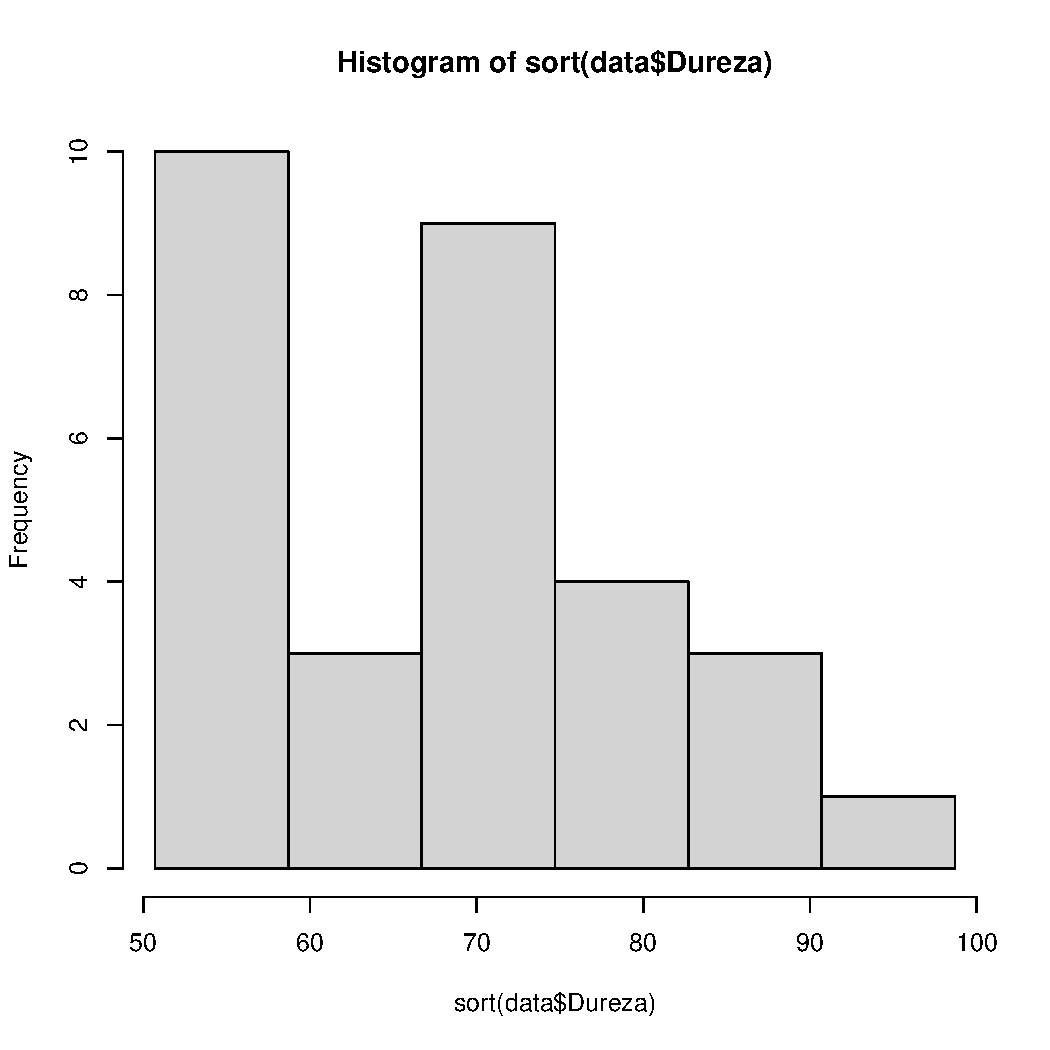
\includegraphics[width=8cm]{./../src/output/03212024_Output_HistogramaDurezaAluminio.pdf}
        \end{figure}
    \end{solution}
    \part Faça o box-plot \footnote{Gráfico que relaciona medidas descritivas: máximo, mínimo, mediana (segundo quartil), primeiro e terceiro quartil} dos dados. Existem outliers \footnote{Valores discrepantes baseados em um limite superior e inferior}?
    \begin{solution}
        Assim teremos:
        \begin{equation*}
            \begin{split}
                max & = 95.4 \\
                min & = 50.7 \\
            \end{split}
        \end{equation*}

        Primeiro quartil $Q_{0.25}$:
        \begin{equation*}
            \begin{split}
                p_{25}              & = 0.25 \times (29 +1) = 0.25 \times 30 = 7.5 \\
                \therefore Q_{0.25} & \in [x_7, x_8]                               \\
                \therefore Q_{0.25} & = 0.5 \times 54.1 + 0.5 \times 55.3 = 54.7
            \end{split}
        \end{equation*}

        Segundo quartil (mediana) $Q_{0.50} = M_d$:
        \begin{equation*}
            \begin{split}
                p_{50}              & = 0.50 \times (29 +1) = 0.50 \times 30 = 15 \\
                \therefore Q_{0.50} & = x_{15} = 69.5                             \\
            \end{split}
        \end{equation*}

        Terceiro quartil $Q_{0.75}$:
        \begin{equation*}
            \begin{split}
                p_{75}              & = 0.75 \times (29 +1) = 0.75 \times 30 = 22.5 \\
                \therefore Q_{0.75} & \in [x_{22}, x_{23}]                          \\
                \therefore Q_{0.75} & = 0.5 \times 77.8 + 0.5 \times 78.5 = 78.15
            \end{split}
        \end{equation*}

        Assim temos o box-plot:
        \begin{figure}[H]
            \centering
            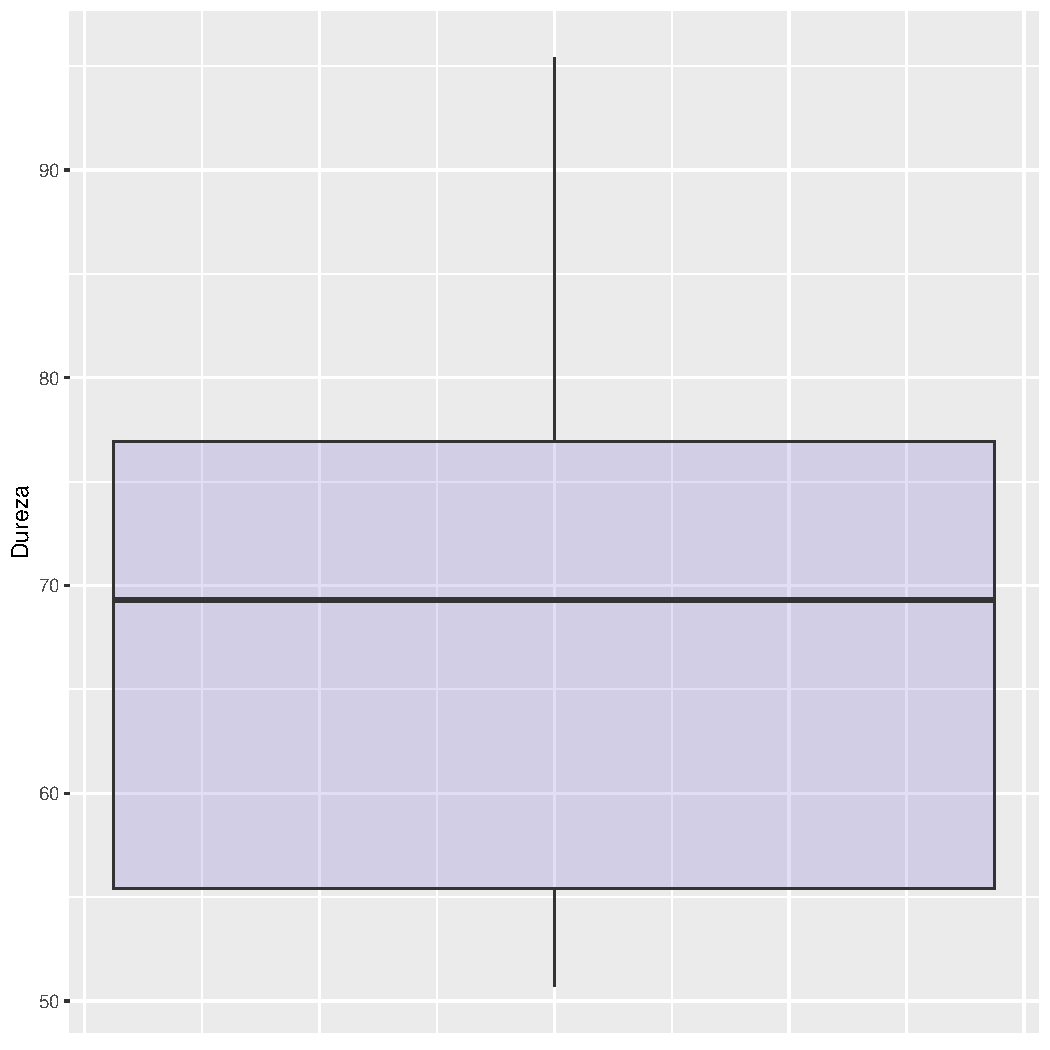
\includegraphics[width=8cm]{./../src/output/03212024_Output_BoxPlotDurezaAluminio.pdf}
        \end{figure}

        Para a análise de \textbf{outliers} temos o \textbf{limite superior} $LS = Q_3 + (1.5)d_q$ e \textbf{limite inferior} $LI = Q_1 - (1.5)d_q$, onde $d_q = Q_3 - Q_1$ ou \textbf{distância interquartil}:
        \begin{equation*}
            \begin{split}
                d_q & = 78.15 - 54.7 = 23.45                                  \\
                LS  & = 78.15 + (1.5 \times 23.45) = 78.15 + 35.175 = 113.325 \\
                LI  & = 54.7 - (1.5 \times 23.45) = 54.7 - 35.175 = 19.525
            \end{split}
        \end{equation*}

        Assim, dado os valores encontrados para $LS$ e $LI$ não temos \textbf{outliers} na amostra.
    \end{solution}
\end{parts}